

\tikzset{every picture/.style={line width=0.75pt}} %set default line width to 0.75pt        

\begin{tikzpicture}[x=0.75pt,y=0.75pt,yscale=-1,xscale=1]
%uncomment if require: \path (0,351); %set diagram left start at 0, and has height of 351

%Image [id:dp7783708648403043] 
\draw (325.8,155.11) node  {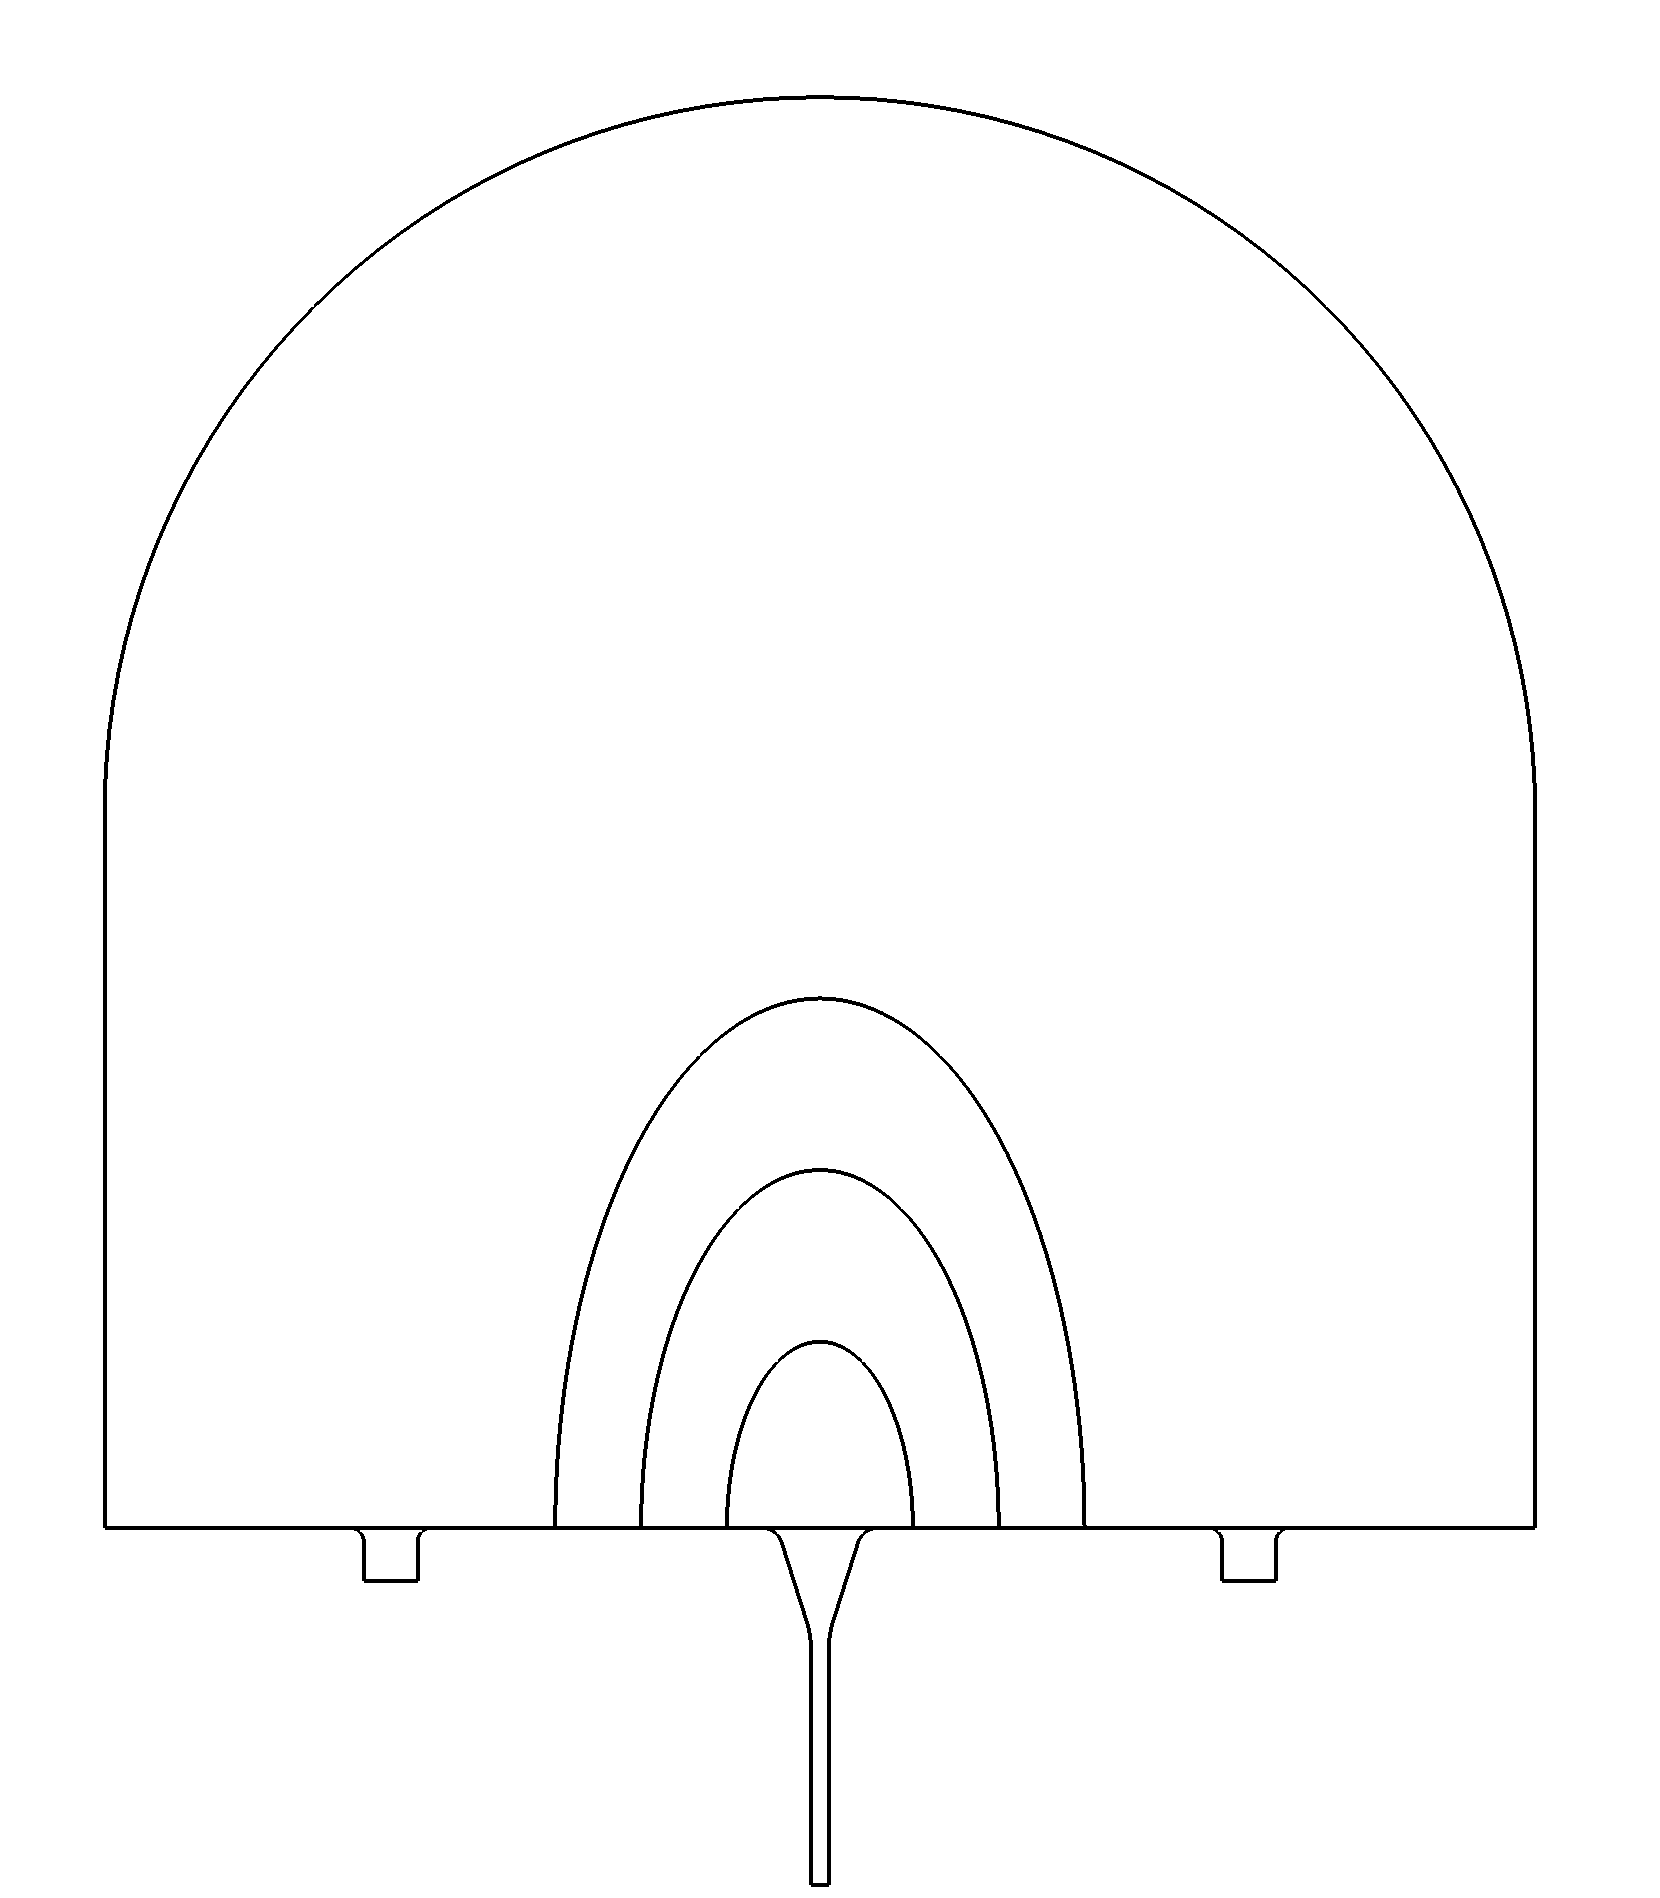
\includegraphics[width=189.6pt,height=216.78pt]{diagrams/placenta-geometry-diagrams/mesh_box-circle.png}};
%Shape: Axis 2D [id:dp020523494814431942] 
\draw  (146.18,293.48) -- (178.98,293.48)(149.46,263.96) -- (149.46,296.76) (171.98,288.48) -- (178.98,293.48) -- (171.98,298.48) (144.46,270.96) -- (149.46,263.96) -- (154.46,270.96)  ;

%Straight Lines [id:da8036713501202459] 
\draw [color={rgb, 255:red, 128; green, 128; blue, 128 }  ,draw opacity=1 ]   (429.5,304.49) -- (219,304.01) ;
\draw [shift={(216,304)}, rotate = 0.13] [fill={rgb, 255:red, 128; green, 128; blue, 128 }  ,fill opacity=1 ][line width=0.08]  [draw opacity=0] (7.14,-3.43) -- (0,0) -- (7.14,3.43) -- cycle    ;
\draw [shift={(432.5,304.5)}, rotate = 180.13] [fill={rgb, 255:red, 128; green, 128; blue, 128 }  ,fill opacity=1 ][line width=0.08]  [draw opacity=0] (7.14,-3.43) -- (0,0) -- (7.14,3.43) -- cycle    ;
%Straight Lines [id:da7908302902450595] 
\draw [color={rgb, 255:red, 155; green, 155; blue, 155 }  ,draw opacity=1 ] [dash pattern={on 0.84pt off 2.51pt}]  (432.5,246.5) -- (432.5,304.5) ;
%Straight Lines [id:da4155602358787114] 
\draw [color={rgb, 255:red, 155; green, 155; blue, 155 }  ,draw opacity=1 ] [dash pattern={on 0.84pt off 2.51pt}]  (216,246) -- (216,304) ;
%Shape: Rectangle [id:dp14174973381317724] 
\draw   (303.75,226.5) -- (343.5,226.5) -- (343.5,300.5) -- (303.75,300.5) -- cycle ;
%Shape: Polygon [id:ds3016551288537974] 
\draw  [fill={rgb, 255:red, 155; green, 155; blue, 155 }  ,fill opacity=0.2 ] (475.75,256.5) -- (343.5,300.5) -- (343.5,226.5) -- (475.75,57) -- cycle ;
%Shape: Rectangle [id:dp9578735364047417] 
\draw  [color={rgb, 255:red, 208; green, 2; blue, 27 }  ,draw opacity=1 ][fill={rgb, 255:red, 255; green, 255; blue, 255 }  ,fill opacity=1 ][line width=2.25] [blur shadow={shadow xshift=0pt,shadow yshift=0pt, shadow blur radius=1.5pt, shadow blur steps=4 ,shadow opacity=100}] (475.75,57) -- (647,57) -- (647,256.5) -- (475.75,256.5) -- cycle ;
%Shape: Rectangle [id:dp23171471463851145] 
\draw   (249.5,238.5) -- (269,238.5) -- (269,256.5) -- (249.5,256.5) -- cycle ;
%Shape: Polygon [id:ds957152197864789] 
\draw  [fill={rgb, 255:red, 155; green, 155; blue, 155 }  ,fill opacity=0.2 ] (249.5,238.5) -- (249.5,256.5) -- (174,154.5) -- (174,59) -- cycle ;
%Shape: Rectangle [id:dp5734000637247996] 
\draw  [color={rgb, 255:red, 74; green, 144; blue, 226 }  ,draw opacity=1 ][fill={rgb, 255:red, 255; green, 255; blue, 255 }  ,fill opacity=1 ][line width=2.25] [blur shadow={shadow xshift=0pt,shadow yshift=0pt, shadow blur radius=1.5pt, shadow blur steps=4 ,shadow opacity=100}] (23.5,59) -- (174,59) -- (174,154.5) -- (23.5,154.5) -- cycle ;
%Image [id:dp7627742527510089] 
\draw (542.33,151) node  {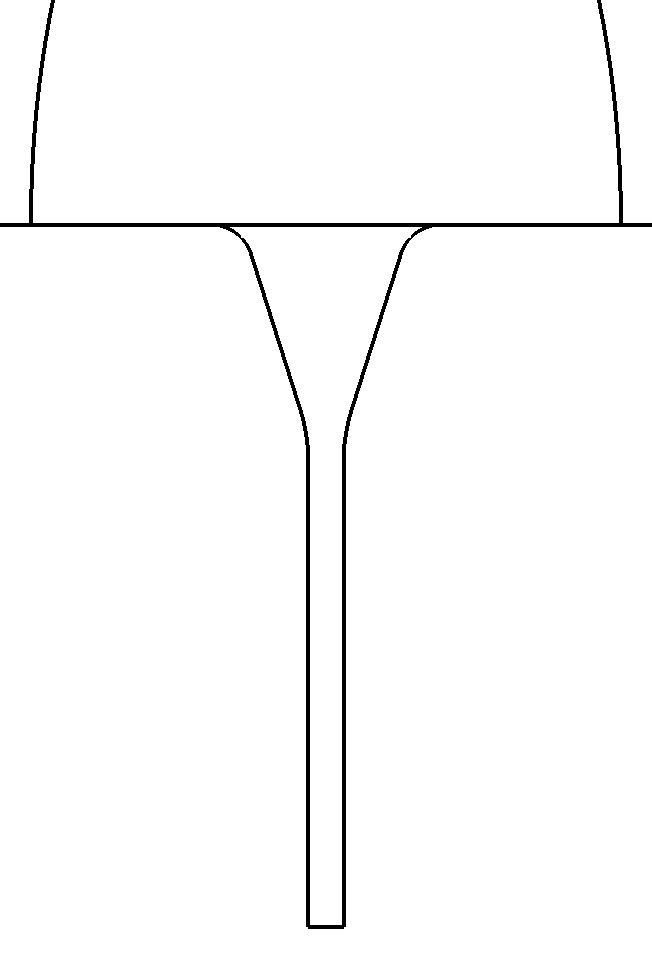
\includegraphics[width=81.5pt,height=121.5pt]{diagrams/placenta-geometry-diagrams/mesh_box-circle_artery.png}};
%Image [id:dp2920261793480039] 
\draw (92.04,105.25) node  {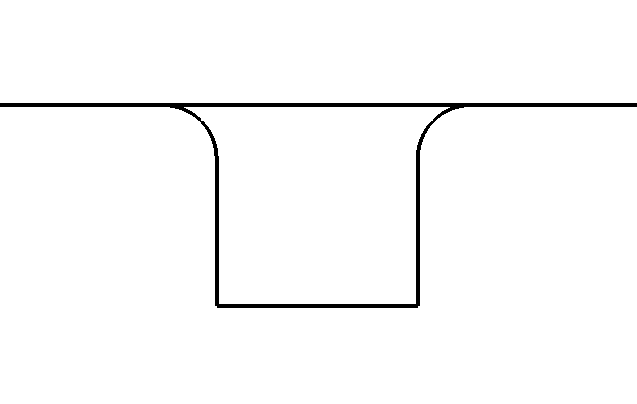
\includegraphics[width=97.56pt,height=61.88pt]{diagrams/placenta-geometry-diagrams/mesh_box-circle_vein.png}};
%Straight Lines [id:da007703491218846725] 
\draw [color={rgb, 255:red, 128; green, 128; blue, 128 }  ,draw opacity=1 ]   (109,130.75) -- (74.75,130.75) ;
\draw [shift={(71.75,130.75)}, rotate = 360] [fill={rgb, 255:red, 128; green, 128; blue, 128 }  ,fill opacity=1 ][line width=0.08]  [draw opacity=0] (5.36,-2.57) -- (0,0) -- (5.36,2.57) -- cycle    ;
\draw [shift={(112,130.75)}, rotate = 180] [fill={rgb, 255:red, 128; green, 128; blue, 128 }  ,fill opacity=1 ][line width=0.08]  [draw opacity=0] (5.36,-2.57) -- (0,0) -- (5.36,2.57) -- cycle    ;
%Straight Lines [id:da6675820105512444] 
\draw [color={rgb, 255:red, 128; green, 128; blue, 128 }  ,draw opacity=1 ]   (122,90.75) -- (122,123.25) ;
\draw [shift={(122,126.25)}, rotate = 270] [fill={rgb, 255:red, 128; green, 128; blue, 128 }  ,fill opacity=1 ][line width=0.08]  [draw opacity=0] (5.36,-2.57) -- (0,0) -- (5.36,2.57) -- cycle    ;
\draw [shift={(122,87.75)}, rotate = 90] [fill={rgb, 255:red, 128; green, 128; blue, 128 }  ,fill opacity=1 ][line width=0.08]  [draw opacity=0] (5.36,-2.57) -- (0,0) -- (5.36,2.57) -- cycle    ;
%Straight Lines [id:da020004946952280278] 
\draw [color={rgb, 255:red, 128; green, 128; blue, 128 }  ,draw opacity=1 ]   (555.5,103) -- (528.25,103) ;
\draw [shift={(525.25,103)}, rotate = 360] [fill={rgb, 255:red, 128; green, 128; blue, 128 }  ,fill opacity=1 ][line width=0.08]  [draw opacity=0] (5.36,-2.57) -- (0,0) -- (5.36,2.57) -- cycle    ;
\draw [shift={(558.5,103)}, rotate = 180] [fill={rgb, 255:red, 128; green, 128; blue, 128 }  ,fill opacity=1 ][line width=0.08]  [draw opacity=0] (5.36,-2.57) -- (0,0) -- (5.36,2.57) -- cycle    ;
%Straight Lines [id:da8088085573407642] 
\draw [color={rgb, 255:red, 155; green, 155; blue, 155 }  ,draw opacity=1 ] [dash pattern={on 0.84pt off 2.51pt}]  (546,144.5) -- (560.75,144.5) ;
%Straight Lines [id:da6668766321328388] 
\draw [color={rgb, 255:red, 155; green, 155; blue, 155 }  ,draw opacity=1 ] [dash pattern={on 0.84pt off 2.51pt}]  (546,224.25) -- (590.75,224.25) ;
%Straight Lines [id:da9239755653729449] 
\draw [color={rgb, 255:red, 128; green, 128; blue, 128 }  ,draw opacity=1 ]   (561.25,141.5) -- (561.25,111) ;
\draw [shift={(561.25,108)}, rotate = 90] [fill={rgb, 255:red, 128; green, 128; blue, 128 }  ,fill opacity=1 ][line width=0.08]  [draw opacity=0] (5.36,-2.57) -- (0,0) -- (5.36,2.57) -- cycle    ;
\draw [shift={(561.25,144.5)}, rotate = 270] [fill={rgb, 255:red, 128; green, 128; blue, 128 }  ,fill opacity=1 ][line width=0.08]  [draw opacity=0] (5.36,-2.57) -- (0,0) -- (5.36,2.57) -- cycle    ;
%Straight Lines [id:da9153150562330312] 
\draw [color={rgb, 255:red, 128; green, 128; blue, 128 }  ,draw opacity=1 ]   (590.75,221.25) -- (590.75,111.25) ;
\draw [shift={(590.75,108.25)}, rotate = 90] [fill={rgb, 255:red, 128; green, 128; blue, 128 }  ,fill opacity=1 ][line width=0.08]  [draw opacity=0] (7.14,-3.43) -- (0,0) -- (7.14,3.43) -- cycle    ;
\draw [shift={(590.75,224.25)}, rotate = 270] [fill={rgb, 255:red, 128; green, 128; blue, 128 }  ,fill opacity=1 ][line width=0.08]  [draw opacity=0] (7.14,-3.43) -- (0,0) -- (7.14,3.43) -- cycle    ;
%Straight Lines [id:da02336395841755401] 
\draw [color={rgb, 255:red, 128; green, 128; blue, 128 }  ,draw opacity=1 ]   (545.25,227.75) -- (539.5,227.75) ;
\draw [shift={(536.5,227.75)}, rotate = 360] [fill={rgb, 255:red, 128; green, 128; blue, 128 }  ,fill opacity=1 ][line width=0.08]  [draw opacity=0] (3.57,-1.72) -- (0,0) -- (3.57,1.72) -- cycle    ;
\draw [shift={(548.25,227.75)}, rotate = 180] [fill={rgb, 255:red, 128; green, 128; blue, 128 }  ,fill opacity=1 ][line width=0.08]  [draw opacity=0] (3.57,-1.72) -- (0,0) -- (3.57,1.72) -- cycle    ;

% Text Node
\draw (182.36,290) node [anchor=west] [inner sep=0.75pt]  [font=\footnotesize]  {$x$};
% Text Node
\draw (150.5,257.55) node [anchor=south] [inner sep=0.75pt]  [font=\footnotesize]  {$y$};
% Text Node
\draw (324.25,307.65) node [anchor=north] [inner sep=0.75pt]  [font=\footnotesize,color={rgb, 255:red, 128; green, 128; blue, 128 }  ,opacity=1 ]  {$40\ \text{mm}$};
% Text Node
\draw (91.88,134.15) node [anchor=north] [inner sep=0.75pt]  [font=\scriptsize,color={rgb, 255:red, 128; green, 128; blue, 128 }  ,opacity=1 ]  {$1.5\ \text{mm}$};
% Text Node
\draw (124,107) node [anchor=west] [inner sep=0.75pt]  [font=\scriptsize,color={rgb, 255:red, 128; green, 128; blue, 128 }  ,opacity=1 ]  {$1.5\ \text{mm}$};
% Text Node
\draw (541.88,99.6) node [anchor=south] [inner sep=0.75pt]  [font=\scriptsize,color={rgb, 255:red, 128; green, 128; blue, 128 }  ,opacity=1 ]  {$2.4\ \text{mm}$};
% Text Node
\draw (563.25,126.25) node [anchor=west] [inner sep=0.75pt]  [font=\tiny,color={rgb, 255:red, 128; green, 128; blue, 128 }  ,opacity=1 ]  {$3\ \text{mm}$};
% Text Node
\draw (592.75,166.25) node [anchor=west] [inner sep=0.75pt]  [font=\scriptsize,color={rgb, 255:red, 128; green, 128; blue, 128 }  ,opacity=1 ]  {$10\ \text{mm}$};
% Text Node
\draw (542.38,232.2) node [anchor=north] [inner sep=0.75pt]  [font=\tiny,color={rgb, 255:red, 128; green, 128; blue, 128 }  ,opacity=1 ]  {$0.5\ \text{mm}$};


\end{tikzpicture}
